\documentclass{jfm-like}
\usepackage{graphicx}
\usepackage{epstopdf, epsfig}

%-------------------------------------------
% additional packages added by KW
%-------------------------------------------
\usepackage{mathrsfs} 
\usepackage{amssymb}
\usepackage{amsmath}
\usepackage{bm}
\usepackage{xcolor}
%-------------------------------------------

\title{A projection method for incompressible flow in domains lacking symmetry}
\shorttitle{Projection in nested domains}
\shortauthor{K. B. Winters}



\author{Kraig Winters
  }

\affiliation{Scripps Institution of Oceanography, University of California San Diego,
La Jolla, CA 92093, USA
}

\begin{document}

\maketitle

% single-paragraph abstract <= 250 words, provides a summary of the main aims and results.
\begin{abstract}
This note documents our approach to nested flow simulations in 2d. The algorithm is designed around fast cosine transforms for differentiation and inversion of the Poisson equation
underlying the projection method. The two fundamental difficulties addressed here are (i) differentiating functions without even or odd symmetry using cosine series and (ii) designing
the projection method so that homogeneous Neumann boundary conditions on the pressure variable are compatible with  inhomogeneous boundary conditions for the velocity field.
\end{abstract}

%\begin{keywords}
%Authors should not enter keywords on the manuscript, as these must be chosen by the author during the online submission process and will then be added during the typesetting process (see http://journals.cambridge.org/data/\linebreak[3]relatedlink/jfm-\linebreak[3]keywords.pdf for the full list)
%\end{keywords}

\section{The problem}
We want to develop techniques for integrating flow solutions in an arbitrary child domain given boundary information derived from a separate, simpler computation of the solution on the parent domain.
To begin, we assume that the same set of governing equations hold throughout both the parent and child domains. An obvious extension is when the equations governing the flow in the parent domain
are simplified, for example by assuming hydrostatic pressure, but the same simplifying assumptions are not enforced in the child domain. While this is an important case, in this note we only consider the
case when the only difference in complexity stems from resolution differences. Here we imagine the flow in the parent domain to be known on a discrete grid of low resolution compared to that of the child domain,
and that the solution in the parent domain can be interpolated in space and time to provide the boundary conditions for flow in the child domain. Figure \ref{fig:schematic} shows the configuration of interest
in two dimensions. The child domain, shown in red, is arbitrarily embedded within a larger parent domain. The boundaries of the domains may or may not coincide, fully or partially. We note that, currently,
nested simulations for ROMS and mitGCM have only been implemented for full-depth child grids. The hope here is to develop a scheme that will enable a much higher resolution child domain to be placed in the upper ocean.
To be fair, however, it should also be noted that both ROMS and mitGCM can be used with grid clustering, subject to mild-variation constraints, thus concentrating effort in the upper ocean if desired.

In this note, we motivate and derive a modified projection algorithm where the underlying numerical engine consists of two-dimensional fast cosine transforms, multiplication using discrete wavenumber arrays, and inverse
transformation. To make the problem amenable to this approach we introduce  semi-analytical modifications to deal with discontinuous derivatives and inhomogeneous boundary conditions without altering the underlying
mathematical problem. In Section 2 we list the governing equations that are taken to be valid over both an outer or parent domain and an arbitrarily nested child domain. In Section 3 we give the explicit analytical
solution for a large-scale near-inertial internal wave mode propagating to the right. Sampling this solution will be used for initial and boundary values used to illustrate the solution procedure in the child domain.
In Section 4.1, we show that the Bernoulli-cosine method can be efficiently used to numerically differentiate data lacking symmetries over a finite domain. In Section 4.2 we derive the projection scheme and explicitly list
the computational steps. We then illustrate the results obtained after each of the key steps along the horizontal and vertical slices through the child domain shown in Figure \ref{fig:schematic}.
In Sectin 5 we discuss the recovery of the physical pressure field and
Aafew closing comments are made in Section 6.
 \begin{figure}
  \centerline{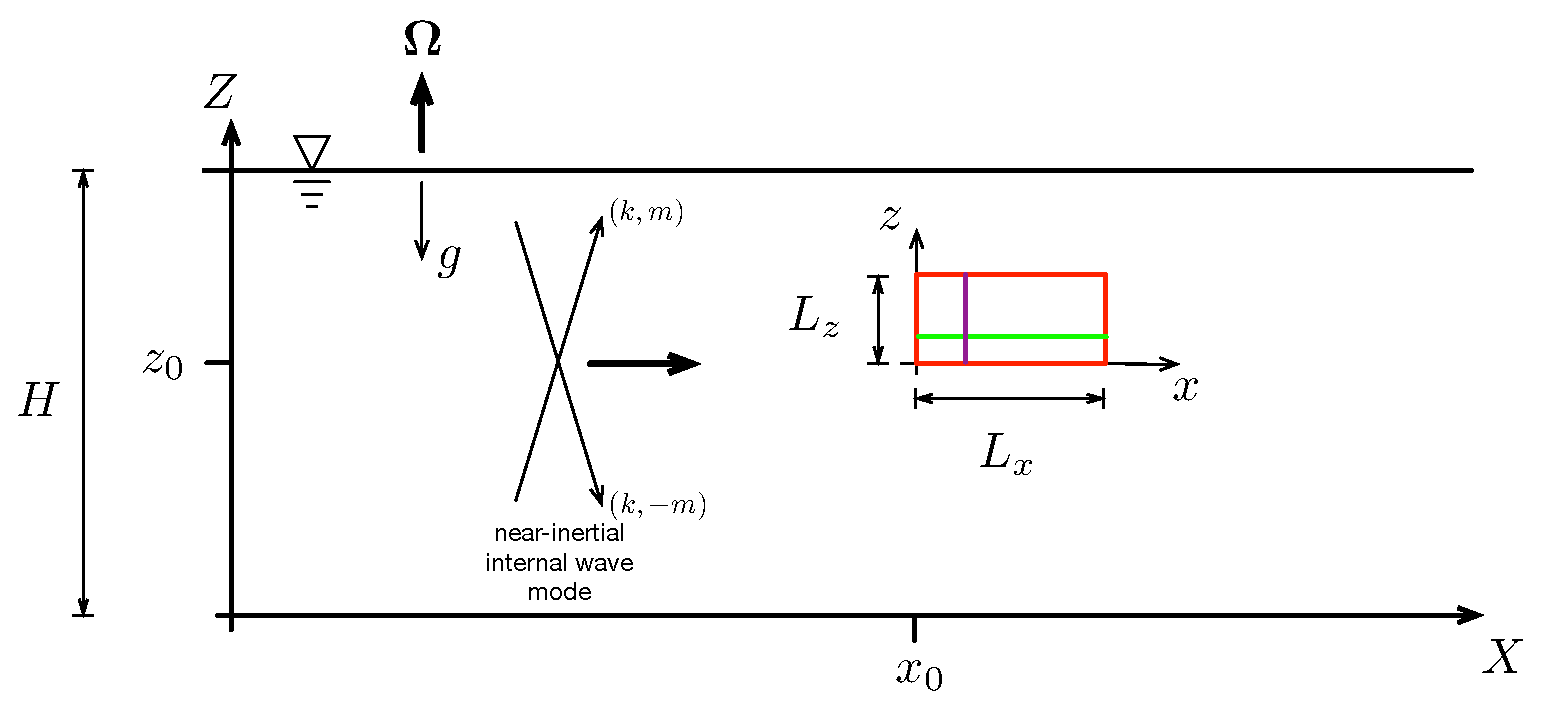
\includegraphics[width=1.0\textwidth]{FIGS/schematic.eps}}
  \caption{Schematic of parent and nested child domains. The child domain is arbitrarily embedded within the parent domain and is shown in red. Slices along which various intermediate results will be shown are indicated in green and purple.} 
  \label{fig:schematic}
\end{figure}

\section{Governing equations}
For both domains we assume the flow is governed by the nonhydrostatic Boussinesq equations on an $f$ plane. For illustration, we assume two-dimensional flow in the $xz$ plane and thus that all $y$ derivatives
are identically zero. For simplicity, we impose free-slip rigid boundaries at $Z=0,H$ and periodicity in $X$ at scale $\mathcal{L}$. Using subscripts to indicate partial derivatives, we write
\begin{equation}
u_t = fv - (u\,u_x + w\,u_z) - {\mathcal D}[u] - p_x
\label{eq:umom}
\end{equation}
\begin{equation}
v_t =  -fu - (u\,v_x + w\,v_z) - {\mathcal D}[v] 
\label{eq:vmom}
\end{equation}
\begin{equation}
w_t =  b  - (u\,w_x + w\,w_z) - {\mathcal D}[w]  - p_z
\label{eq:wmom}
\end{equation}
\begin{equation}
b_t =  -N^2 w  - (u\,b_x + w\,b_z) - {\mathcal D'}[b]  
\label{eq:buoy}
\end{equation}
\begin{equation}
u_x + w_z = 0.
\label{eq:cont}
\end{equation}
Here $[u,v,w]$ are the velocity components in the $x$, $y$ and $z$ directions respectively and $p$ is the perturbation pressure scaled by the reference density $\rho_0$. Density perturbations $\rho'$
are assumed to be small in magnitude and so the Boussinesq approximation has been made along with linearity in the equation of state.
The buoyancy $b=-(g/\rho_0)\rho'$ has been decomposed into its background component $B(z)$ and its perturbation $b$ and $N^2 = B_z$.
The operators ${\mathcal D}$ and  ${\mathcal D'}$ are diffusion operators for momentum and heat respectively.




\section{Known solution in the parent domain}
To illustrate the approach to computing solutions in the child domain, we specify an exact solution to the linearized, inviscid and nondiffusive versions of Eqs. (\ref{eq:umom})-(\ref{eq:cont}) that represents a propagating internal wave mode.
For small wave amplitudes and sufficiently large spatial scales, this parent solution can be regarded as a very good approximation to the full governing equations. Explicitly, with $\theta = kX - \omega t + \psi$,
\begin{equation}
u = A \cos(mZ) \cos(\theta) ~,~ v = A \frac{f}{\omega} \cos(mZ) \sin(\theta) ~,~ w = A \frac{k}{m} \sin(mZ) \sin(\theta)
\label{eq:usoln}
\end{equation}
\begin{equation}
 b = -A  \frac{k}{m} \frac{N^2}{\omega} \sin(mZ) \cos(\theta) ~,~ p = A \frac{\omega^2-f^2}{k \omega} \cos(mZ) \cos(\theta).
\label{eq:bpsoln}
\end{equation}
The frequency $\omega$ satisfies the dispersion relation
\begin{equation}
\omega^2 = \frac{k^2 N^2 + m^2 f^2}{k^2 + m^2}
\end{equation}
and $\psi$ is an arbitrary phase shift.
To satisfy the boundary conditions in the parent domain we take $m \in (\pi/H) \left\{ 1,2, \dots \right\}$ and  $k \in (2\pi/{\mathcal L}) \left\{ 1,2, \dots \right\}$.
Within the child domain, the parent solutions (\ref{eq:usoln}) and (\ref{eq:bpsoln})  are easily available as needed using the shifted coordinates $X=x + x_0$ and $Z=z + z_0$.


\section{Overall approach}
We want to compute solutions to the governing equations in the child domain, taking initial conditions and boundary information from previously computed (or in this case known) solutions
from the parent domain. We want the solution techniques to be as close as possible to the solver ${\bf flow\_solve}$ which relies on fast trigonometric transforms for efficient, accurate differentiation and
and solution of the Poisson equation for pressure. The difficulty to be overcome is that, within the child domain, the desired solutions obey no particular symmetries and so it is not obvious
how series expansions in terms of trigonometric basis functions can be employed. Nevertheless, we persevere and insist on formulating the algorithm around cosine expansions, fast transform differentiation,
and fast transform inversion of the pressure equation. Many of the technical details are discussed  in the separate notes {\em Healing discontinuous derivatives with low-order Bernoulli polynomials}
and {\em Modeling the open-boundary approach to pressure projection}.

\subsection{Fast Bernoulli-cosine differentiation}
This problem requires  the calculation of discrete derivatives of data given on finite domains with no particular symmetries. Such data can always be even-extended into a domain of twice the length to form
a periodic function amenable to representation in a Fourier series expansion. This is formally equivalent to a cosine series expansion of the original data. The fundamental problem is that the even-extended
function has discontinuous derivatives at the end and midpoints of the extended domain. These discontinuities give rise to Gibbs oscillations when the cosine series is differentiated term by term. 

Our approach is the following.
We construct a series expansion using Bernoulli polynomials expanded about the singular points. Requiring these series to match the given data at a few nearby grid points yields an analytically
known function (given the expansion coefficients) that matches the discontinuous structure of the original function. Subtraction of this function from the original leaves behind a smooth, differentiable
function that can be differentiated using standard term by term differentiation of its cosine transform. The Bernoulli polynomial series is analytically differentiable and so the desired derivative
is obtained by combining the two. The details of this approach are described in the notes {\em Healing discontinuous derivatives with low-order Bernoulli polynomials}.

Figure \ref{fig:trig} shows an example of this approach for a phase shifted sinusoidal function on $x \in [0,L]$ that is neither even nor odd. Term by term differentiation of the cosine series
yields a derivative estimate that suffers from large Gibbs oscillations near the end points (shown in blue) as well as small-amplitude, high-wavenumber contamination in the interior. 
Decomposing the function into two low-order Bernoulli polynomial series and a well-behaved residual allows
very accurate computation of the derivative. The normalized error between the exact derivative and that obtained using a 4-term series expansion and 129 grid points is also shown in the figure.
 \begin{figure}
  \centerline{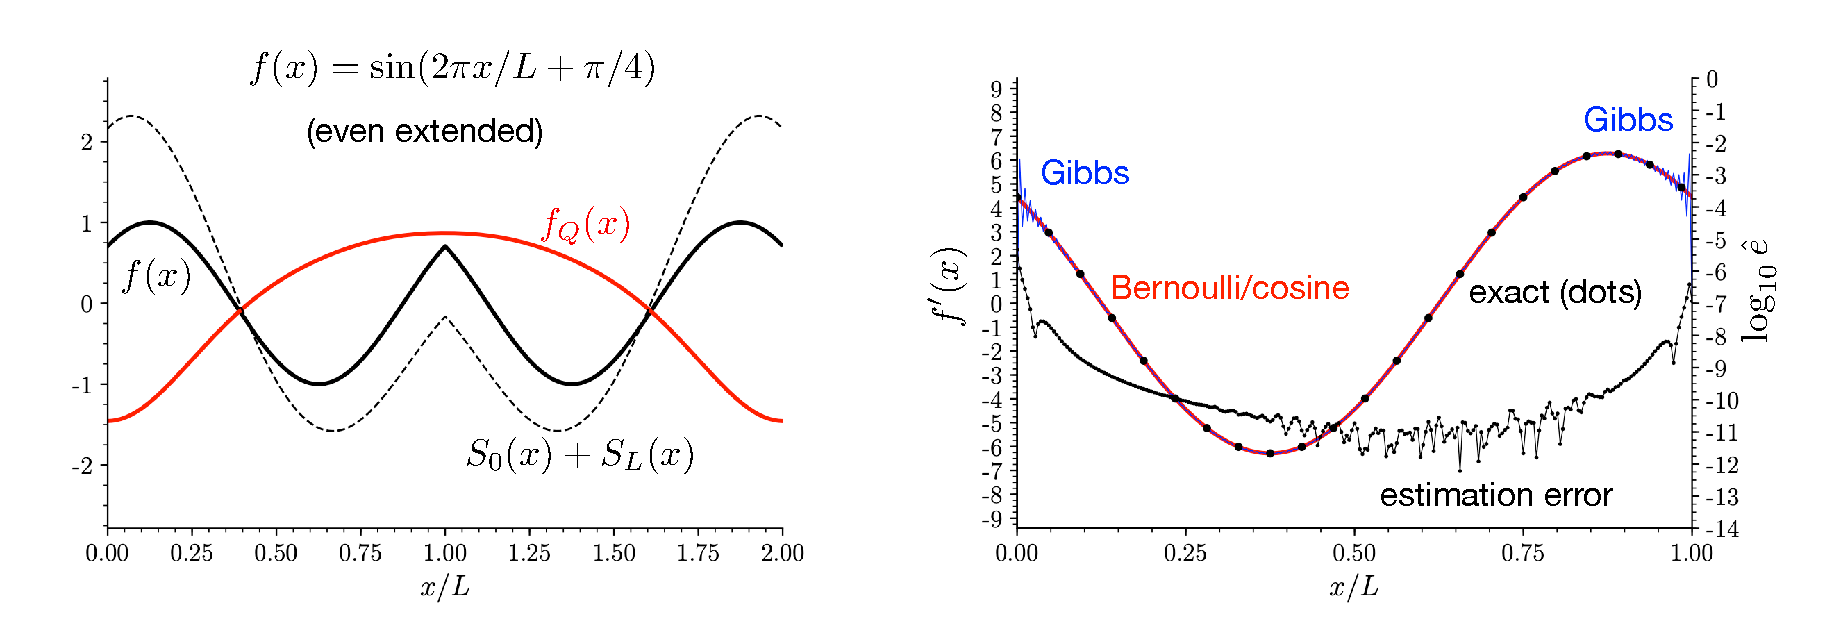
\includegraphics[width=1.0\textwidth]{../differentiation_w_Bernoulli/FIGS/trig_figs/trig_fig.eps}}
  \caption{Explicit Bernoulli-cosine differentiation example for $f(x)=\sin(2\pi x/L + \pi/4)$ using 4 term series expansions. (a) The function $f(x)$, the analytically differentiable series $S_0(x)+S_L(x)$ and the 
  difference $f_Q(x)$ which is amenable to term by term differentiation of its cosine series.}
   \label{fig:trig}
\end{figure}

This decomposition of the data is computationally inexpensive. In this example (Bernoulli polynomial orders of 2,4,6 and 8), 
computing the expansion coefficients requires the solution of two 4x4 matrix problems where the coefficient matrices can be formed and factored
as a preprocessing task. The right hand sides for these problems are simply  4 function values taken near the singular points. Given the expansion coefficients, the series are directly summed using the lowest few
even (periodic, shifted about the singular points) Bernoulli polynomials. These can be evaluated on the discrete set of grid points once, as part of the preprocessing, and saved for repeated use. The operation count for constructing and subtracting
the series is O(N), where N is the number of discrete grid points. Since cosine transform differentiation is O(N log N), this technique is inexpensive in comparison.


\subsection{Incompressibility by projection}
To define the projection scheme, it is convenient to simplify notation and rewrite Eqs. (\ref{eq:umom}) and (\ref{eq:wmom}) as
\begin{equation}
u_t = {\mathcal R}_1 - p_x
\label{eq:umom2}
\end{equation}
\begin{equation}
w_t =   {\mathcal R}_3 - p_z
\label{eq:wmom2}
\end{equation}
where ${\mathcal R}_1$  and ${\mathcal R}_3$ denote all the terms except the pressure gradient on the right-hand side of the $x$ and $z$ momentum equations respectively. 
Integrating in time from $t^n$ to $t^{n+1}$ gives
\begin{equation}
u^{n+1} = u^{n}  + \int_{t^n}^{t^{n+1}}  {\mathcal R}_1  \,{\rm d}t  - \Delta t \, P_x
\label{eq:umom3}
\end{equation}
\begin{equation}
w^{n+1} = w^{n}  + \int_{t^n}^{t^{n+1}}  {\mathcal R}_3 \, {\rm d}t  - \Delta t \, P_z
\label{eq:wmom3}
\end{equation}
where $P$ is the average value of $p$ over the time step. Though we will estimate the time integrals using discrete approximations (4th order Adams Bashforth for example), 
it is convenient to work with them in their exact, continuous form.
Let
\begin{equation}
u_* = u^{n}  + \int_{t^n}^{t^{n+1}}  {\mathcal R}_1  \,{\rm d}t  ~~{\rm and}~~ w_* = w^{n}  + \int_{t^n}^{t^{n+1}}  {\mathcal R}_3  \,{\rm d}t.
\label{eq:ustardefs}
\end{equation}
Then
\begin{equation}
u^{n+1} = u_* - \Delta t \, P_x
\label{eq:umom4}
\end{equation}
\begin{equation}
w^{n+1} = w_* - \Delta t \, P_z.
\label{eq:wmom4}
\end{equation}

Taking the two-dimensional divergence and imposing Eq. (\ref{eq:cont}) on the $t^{n+1}$ velocity gives a Poisson equation for the (time-averaged) pressure $P$:
\begin{equation}
\nabla^2 P = \frac{1}{\Delta t} \nabla \cdot {\vec u}_* 
\label{eq:poisson1}
\end{equation}
where $ {\vec u}_* $ is the vector with components $u_*$ and $w_*$.
Taking the dot product of Eqs. (\ref{eq:umom4}) and  (\ref{eq:wmom4}) with the outward facing unit normal ${\hat n}$ yields the boundary conditions
\begin{equation}
\frac{\partial P}{\partial n} = \frac{1}{\Delta t} ( {\vec u_*} - {\vec u^{\,n+1}} ) \cdot {\hat n}.
\end{equation}
If $ {\vec u_*} \cdot {\hat n}$ were to match $ {\vec u}^{\,n+1} \cdot {\hat n}$ on the boundaries, then the right hand side of this equation would vanish and the required boundary condition for $\frac{\partial P}{\partial n}$ would be homogeneous.
In this case  a solution based on cosine transformations would
be appropriate. (See the notes {\em Modeling the open-boundary approach to pressure projection} for a discussion of inverting the Poisson equation when the source term has discontinuous derivatives.)
Unfortunately, for general boundary conditions,  and in particular for  boundary values ${\vec u^{\,n+1}}$ supplied on the boundary of a nested domain like that in Figure \ref{fig:schematic}, the Neumann
condition is inhomogeneous. The strategy we will adopt is to modify the elliptic equation to one that has homogeneous Neumann boundary conditions.

 We introduce functions $\psi_u(x,z)$, $\psi_w(x,z)$ and $\Psi(x,z)$ such that
\begin{equation}
u^{n+1} = (u_*+  \psi_u) - \Delta t \, (P_x + \Psi_x)
\label{eq:umom5}
\end{equation}
\begin{equation}
w^{n+1} = (w_* + \psi_w)  - \Delta t \, ( P_z + \Psi_z)
\label{eq:wmom5}
\end{equation}
and note that these equations are identical to (\ref{eq:umom4}) and  (\ref{eq:wmom4}) provided that
\begin{equation}
\Delta t \, \nabla \Psi = [\psi_u,\psi_w] = {\vec \psi}.
\end{equation}
Let ${\hat P} = P + \Psi$ be the pressure projection variable,  ${\hat u_*} = (u_*+  \psi_u)$ and ${\hat w_*} = (w_*+  \psi_w)$. Then
\begin{equation}
u^{n+1} = {\hat u_*} - \Delta t \, {\hat P} _x
\label{eq:umom6}
\end{equation}
\begin{equation}
w^{n+1} =  {\hat w_*} - \Delta t \, {\hat P} _z
\label{eq:wmom6}
\end{equation}
and
\begin{equation}
\nabla^2 {\hat P}  = \frac{1}{\Delta t} \nabla \cdot {\vec {\hat u}}_* .
\label{eq:poisson2}
\end{equation}
Provided that ${\vec \psi}$ is any smooth function that satisfies
\begin{equation}
{\vec \psi} \cdot {\hat n} =  ( {\vec u^{\,n+1}} - {\vec u_*} ) \cdot {\hat n}
\label{eq:normal_bcs}
\end{equation}
on the boundaries, the required boundary conditions for ${\hat P}$ are simply
\begin{equation}
\frac{\partial {\hat P}}{\partial n} = 0.
\label{eq:poissonbcs2}
\end{equation}
The Poisson equation for ${\hat P}$ with homogeneous Neumann boundary conditions can now be efficiently solved using a standard cosine transform approach.

\vspace{14pt}
\noindent{\bf Normal components of velocity:} We now construct ${\vec \psi} = [\psi_u,\psi_w]^{\perp}$ so that Eq. (\ref{eq:normal_bcs}) is satisfied. 
The superscript indicates that this function is introduced to enforce boundary conditions on the velocity components normal to the boundaries.
For example,
\begin{equation}
\psi_u(x,z)^{\perp} = A_1(z) \, e^{-[x/\gamma_x]^2} +  A_2(z) \, e^{-[(x-L_x)/\gamma_x]^2} 
\label{eq:ustar_normal_correction}
\end{equation}
where 
$$A_1(z) = u^{n+1}(0,z) - u_*(0,z) $$ and 
$$A_2(z) = u^{n+1}(L_x,z) - u_*(L_x,z)$$
satisfies the required conditions in the limit $L_x \to \infty$ for any $\gamma_x>0$.
Small errors of order $e^{-[L_x/\gamma_x]^2}$ are made for finite $L_x$. There is a tradeoff between
the magnitude of the errors at the endpoints and the difficulty in numerically resolving $\psi^\perp$. In practice,
choosing $\gamma_x \approx L_x/8$ renders $\psi^\perp$ easily resolvable throughout the domain with negligible endpoint errors
on the order of $e^{-8^2} \approx 10^{-28}$.

Similarly, for any $x$ we define
\begin{equation}
\psi_w(x,z)^{\perp} = B_1(x) \, e^{-[z/\gamma_z]^2} +  B_2(x) \, e^{-[(z-L_z)/\gamma_z]^2} 
\label{eq:wstar_normal_correction}
\end{equation}
where $B_1(x) = w^{n+1}(x,0) - w_*(x,0) $ and $B_2(x) = w^{n+1}(x,L_z) - w_*(x,L_z)$.

\vspace{14pt}
\noindent{\bf Tangential components of velocity:} 
Consider the behavior of the tangential flow adjacent to the boundaries, for example $w^{n+1}$ near $x=0$. Eq. (\ref{eq:wmom6}) shows that $w^{n+1}$ at the left boundary will depend
on what we choose to prescribe for $\psi_w$ but also on ${\hat P}_z$, which is an unknown part of the solution to the Poisson equation with homogeneous Neumann boundary conditions. We are not free to constrain
tangential derivatives of ${\hat P}$ at the boundaries. 

Differentiating Eq. (\ref{eq:wmom6}) with respect to $x$, however, eliminates the pressure term because $\frac{\partial}{\partial n}{\hat P} = 0$ at the boundaries. Therefore, we can augment $\psi_w$ with
a  function that ensures that ${\hat w}_x \to w_x^{n+1}$ as $x \to 0,L_x$ from the interior of the domain. To maintain satisfaction of Eq.(\ref{eq:normal_bcs}), however, we do not apply this correction {\em at} normally oriented boundaries
but rather, we rely on smoothness of the solution and the intermediate quantities derived in the neighborhood of the boundaries to yield well-posed constraints. 
We can define, for example,
\begin{equation}
\psi^{\parallel}_w(x,z) = C_1(z) e^{-x/\gamma_x} + C_2(z) e^{-(L_x-x)/\gamma_x}
\end{equation}
%gamma_x*( -W_x - ddn_w )
where $$C_1(z) = \gamma_x \left( w_x^{n+1}(0,z) - \frac{\partial}{\partial n} \left[ w_*(0,z) - \psi^{\perp}_w(0,z) \right] \right )$$ and
 $$C_2(z) = \gamma_x \left( w_x^{n+1}(L_x,z) - \frac{\partial}{\partial n} \left[ w_*(L_x,z) - \psi^{\perp}_w(L_x,z) \right] \right) $$.
 
 Similarly, 
\begin{equation}
\psi^{\parallel}_u(x,z) = D_1(x) e^{-z/\gamma_z} + D_2(x) e^{-(L_z-z)/\gamma_z}
\label{eq:psipar}
\end{equation}
where $$D_1(z) = \gamma_z \left( u_z^{n+1}(x,0) - \frac{\partial}{\partial n} \left[ u_*(x,0) - \psi^{\perp}_u(x,0) \right] \right )$$ and
 $$D_2(z) = \gamma_z \left( u_z^{n+1}(x,L_z) - \frac{\partial}{\partial n} \left[ u_*(x,L_z) - \psi^{\perp}_u(x,L_z) \right] \right) $$.

\vspace{14pt}
\noindent{\bf Recipe for pressure projection:} 
We can now explicitly specify the steps for a projection algorithm to solve for incompressible, rotating stratified flow in domains where boundary information is available-- such as the nested subdomain shown in
Figure \ref{fig:schematic}. The algorithm exploits cosine transform techniques for efficiency and accuracy, augmented by computationally inexpensive low-order expansions in even Bernoulli polynomials to mitigate
discontinuous derivatives for functions lacking symmetry.  It can be coded using the same data transpose routines used in periodic domains or for problems with even or odd symmetries.
The recipe is given below.
\vspace{14pt}

\fcolorbox{black}[HTML]{E9F0E9}{\parbox{\textwidth}{%
\noindent \textbf{Projection algorithm for incompressible flow:}
\vspace{14pt}
\begin{enumerate}
\setlength\itemsep{1em}
\item Given $[u,v,w,b]^{n}$, compute $[v,b]^{n+1}$ from Eqs. (\ref{eq:vmom}) and (\ref{eq:buoy}) using an explicit, discrete time stepping scheme and the Bernoulli-cosine method for discrete spatial differentiation.
At the boundaries, insert the known values of  $[v,b]^{n+1}$.
\item Given $[u,v,w,b]^{n}$, compute $[u_*,w_*]$ from Eq. (\ref{eq:ustardefs}) using an explicit, discrete time stepping scheme and the Bernoulli-cosine method for discrete spatial differentiation.
\item Given boundary information for $[u,v,w,b]^{n+1}$, compute ${\hat u}_* = u_* + \psi^\perp_u +  \psi^\parallel_u,$ and ${\hat w}_* = w_* + \psi^\perp_w +  \psi^\parallel_w$ using 
Eqs. (\ref{eq:ustar_normal_correction})-(\ref{eq:psipar}).
\item Compute the source term in Eq.(\ref{eq:poisson2}) using the Bernoulli-cosine method for spatial differentiation.
\item Compute the two-dimensional cosine transform of the source term and multiply by the wavenumber array $-1/(k_i^2 + m_j^2)$. Set the mean component to zero and inverse transform to get ${\hat P}(x,z)$ satisfying
Eqs. (\ref{eq:poisson2}) and  (\ref{eq:poissonbcs2}).
\item Compute $\nabla {\hat P}$ using the standard term by term differentiation of its two-dimensional cosine series expansion.
\item Project ${\hat u}_*$ and ${\hat w}_*$ onto their divergence-free subspace using Eqs. (\ref{eq:umom6}) and (\ref{eq:wmom6}).
\end{enumerate}
\vspace{14pt}
}}

\vspace{14pt}
After step (c), the functions ${\hat u}_*(x,z)$ and ${\hat w}_*(x,z)$ have been constructed. Figure \ref{fig:projection_slices} shows slices of these functions taken from the green and purple lines in Figure \ref{fig:schematic}
for the outer problem defined in Section 3 with $x_0= .5 {\mathcal L}$, $z_0=0.6\,H$,  $L_x= {\mathcal L}/5$ and $L_z= H/5$. In the subdomain, 129 grid points were used in both the $x$ and $z$ directions and
 $\Delta t$ was set to $(2\pi/\omega)/129$. At the endpoints $x=0$ and $x=L_x$ we require that $u_*$ match the known boundary values for the normal velocity component $u^{\,n+1}$. The red circles in panel (a) highlight that these conditions are satisfied.
The tangential boundary conditions require that the normal derivatives of ${\hat w}_*$ converge to those of $w^{\,n+1}$ at  $x=0$ and $x=L_x$. The black circles in panel (a) highlight that these conditions are also satisfied.
 Panel (b) shows the same quantities along a vertical slice with $x=L_x/4$. Satisfaction of the boundary conditions  for the normal components of velocity at $z=0$ and $L_z$ are highlighted with black circles while those for the
 tangential components with red.
  \begin{figure}
  \centerline{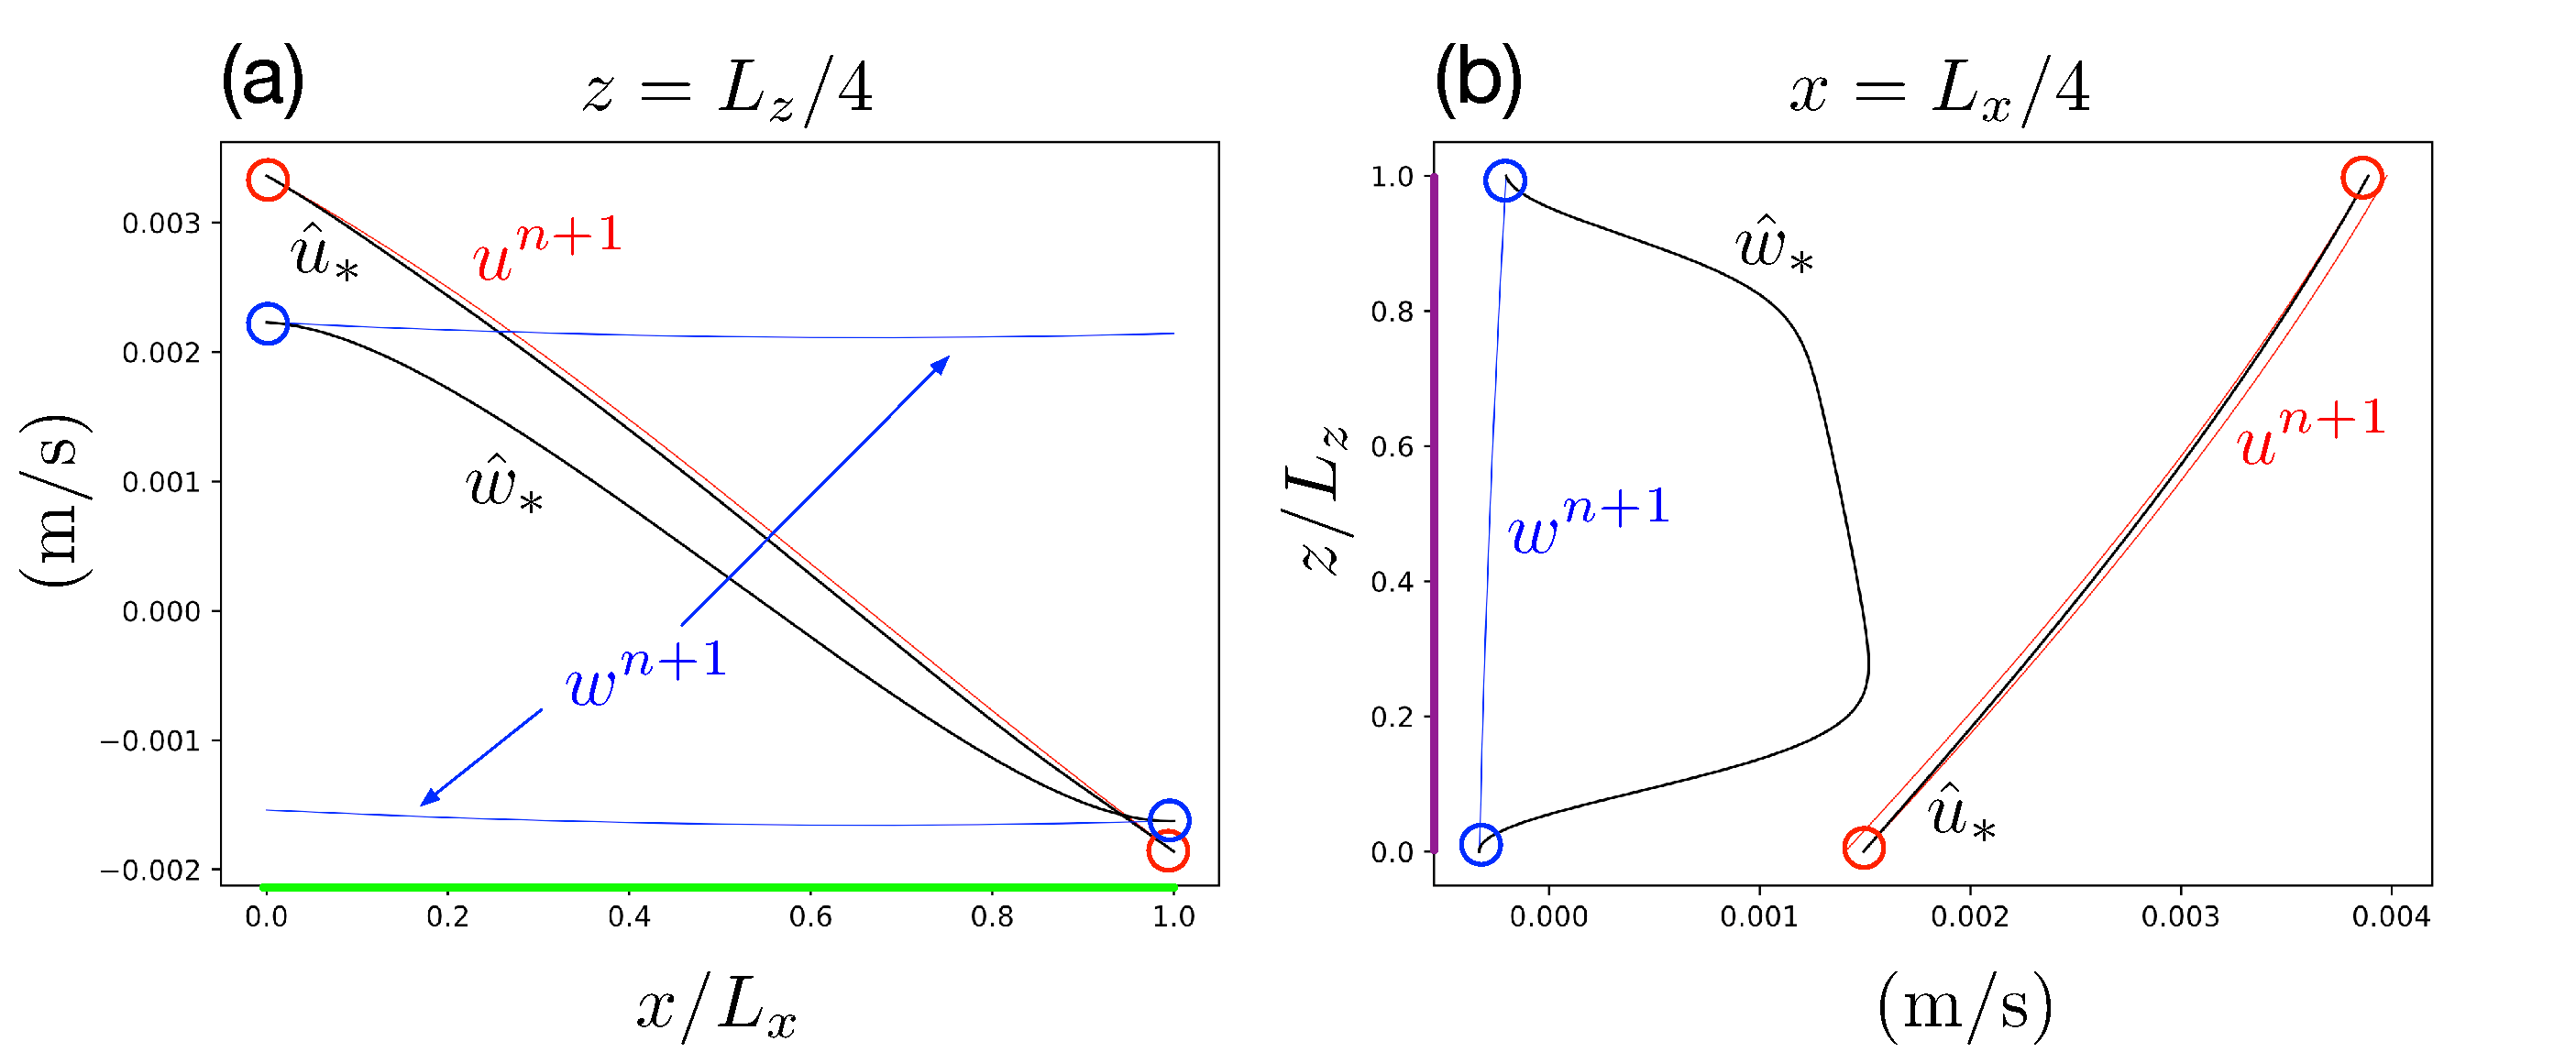
\includegraphics[width=1.0\textwidth]{FIGS/projection_slices.eps}}
  \caption{(a) The exact solutions $u^{n+1}(x)$ (red) and $w^{n+1}(x)$ (blue, shown with two vertical offsets for illustration) at $z=L_z/4$, {\em i.e.} along the green line in Figure \ref{fig:schematic}. 
  Also shown are the functions ${\hat u}_*(x)$ and  ${\hat w}_*(x)$ taken along the same line.
  (b) The exact solutions $u^{n+1}(z)$ (red,  shown with two horizontal offsets for illustration) and $w^{n+1}(z)$ (blue) at $x=L_x/4$, {\em i.e.} along the purple line in Figure \ref{fig:schematic}. 
  Also shown are the functions ${\hat u}_*(z)$ and  ${\hat w}_*(z)$ taken along the same line.} 
  \label{fig:projection_slices}
\end{figure}


In step (d) we compute the divergence of ${\vec {\hat u}_*}$. Because ${\hat u}_*$ and ${\hat w}_*$ have no particular symmetries, the derivatives are computed using the Bernoulli-cosine method. The results are shown 
in Figure \ref{fig:divustarhat} along the same slices
as in Figure \ref{fig:projection_slices} and are well-behaved near the boundaries as expected. The even extension of the divergence into $[0,2L_x) \times [0,2L_z)$ is continuous but has discontinuous derivatives. 
 \begin{figure}
  \centerline{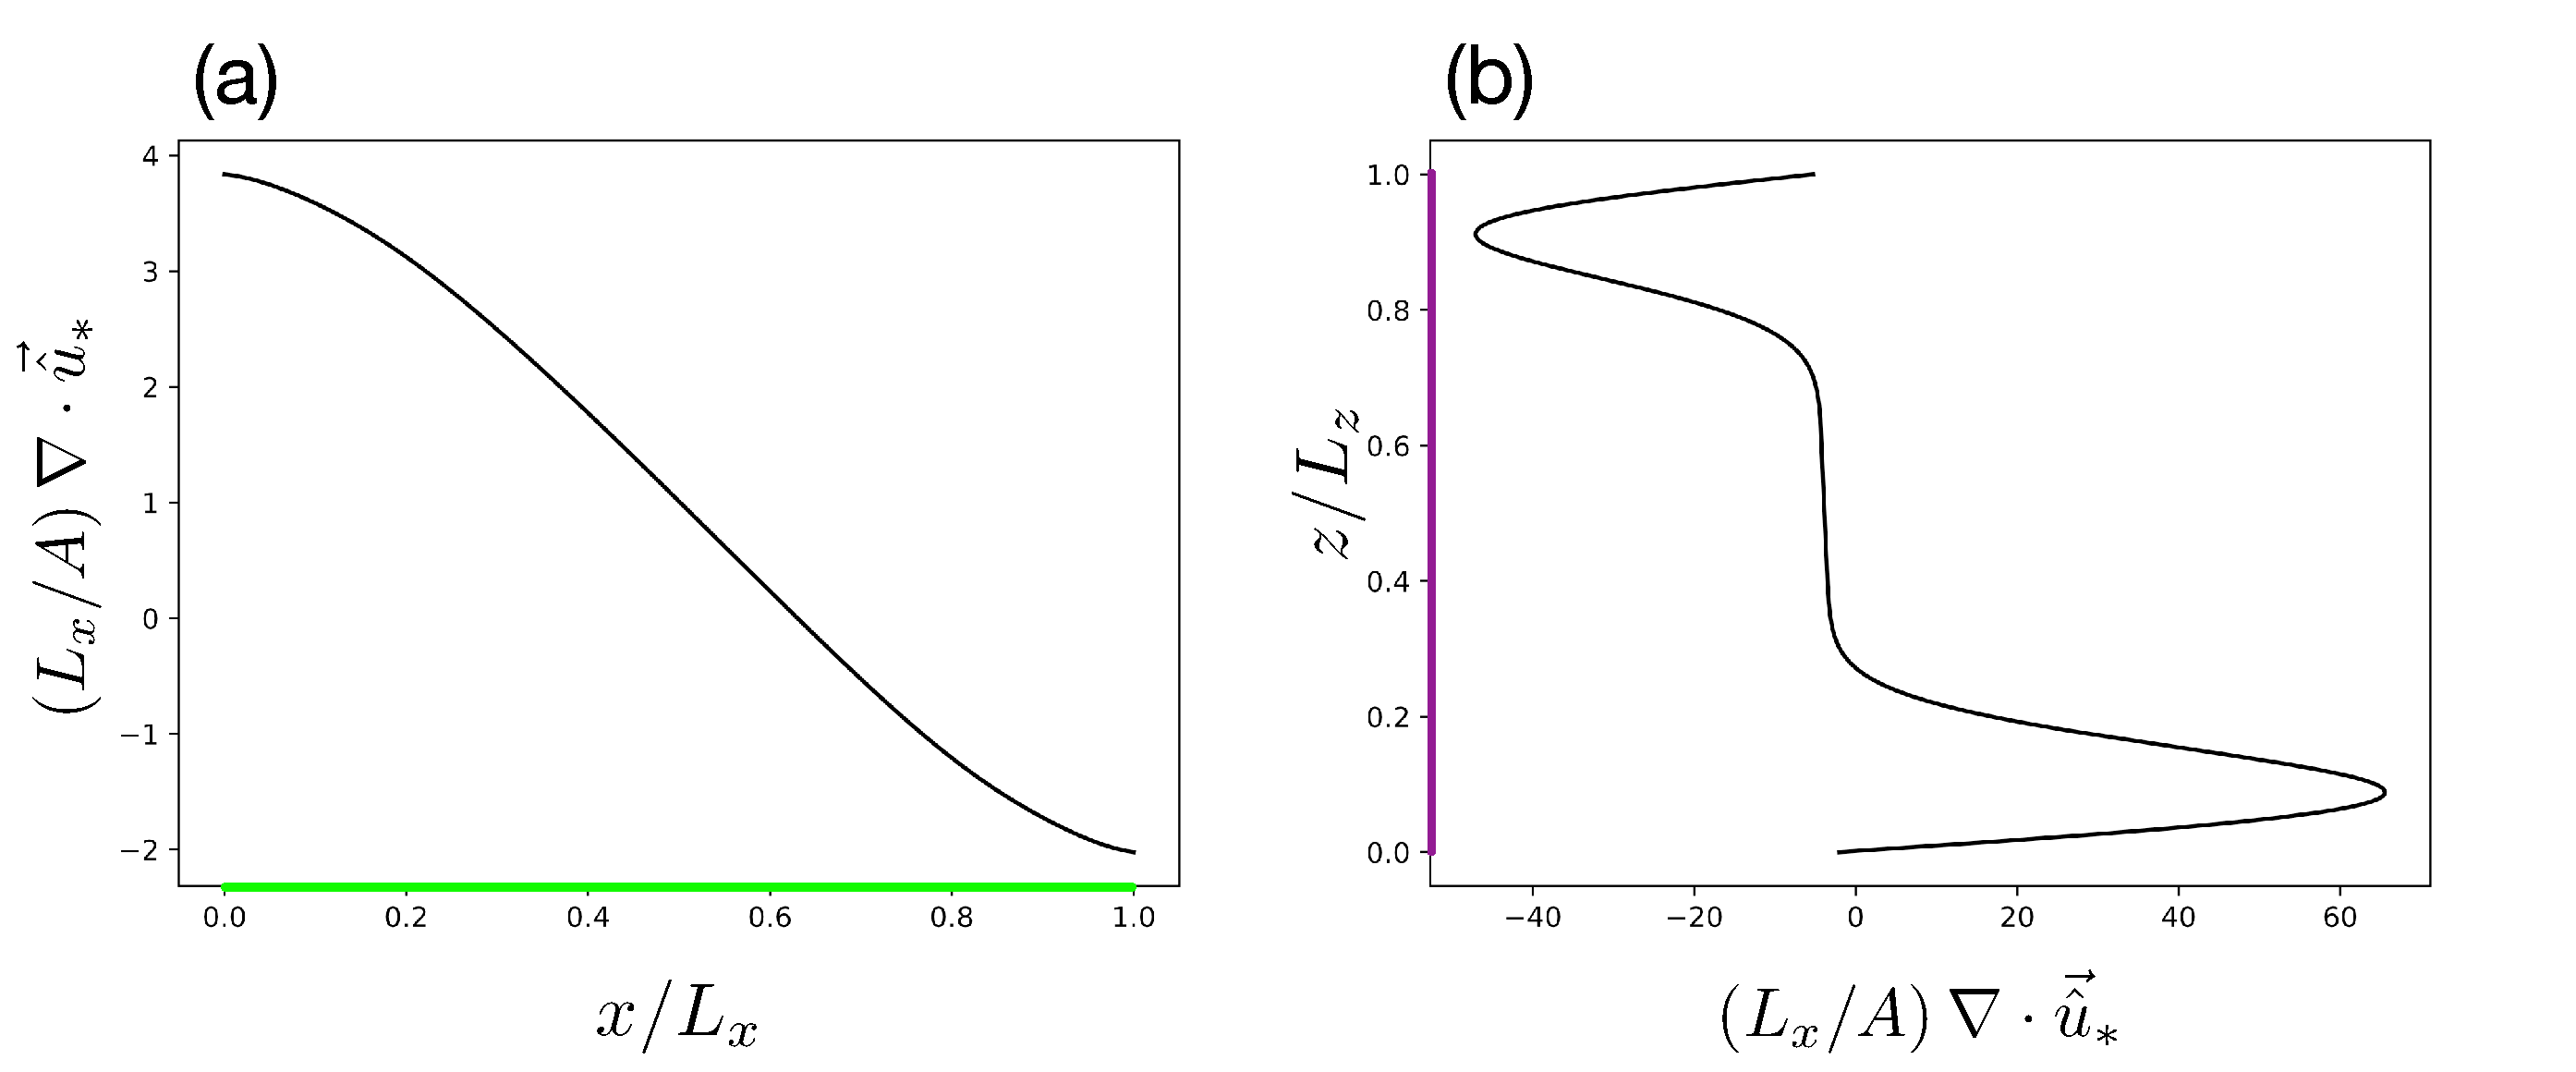
\includegraphics[width=1.0\textwidth]{FIGS/divustarhat.eps}}
  \caption{The divergence of ${\vec {\hat u}_*}$ at $z=L_z/4$ (a) and at $x=L_x/4$ (b). }
  \label{fig:divustarhat}
\end{figure}

The computed divergence of ${\vec {\hat u}_*}$ is amenable
to expansion in cosine series,  multiplication of the coefficients by the discrete wavenumber array $-1/(k_i^2+m_j^2)$, and inversion. The compatibility condition for the homogeneous Neumann boundary conditions
is enforced by setting the (0,0) wavenumber component to zero. The resulting field ${\hat P}$, shown in Figure \ref{fig:phat_p}, is well behaved and continuously differentiable. The  analytical solution for the true pressure $p$, evaluated from Eq. (\ref{eq:bpsoln}) at $t^{\,n+1}$, is also shown for comparison. The two variables differ by the function $\Psi$ due to the augmentation of ${\vec u}_*$ with $\vec \psi$ (see Eqs. (\ref{eq:umom5}) and  (\ref{eq:wmom5})). By design, the difference
is intended to shift the intrinsic inhomogeneity of the boundary conditions for $P$ to the source term for ${\hat P}$ where it can be more easily handled numerically without changing the underlying mathematical problem.
 \begin{figure}
  \centerline{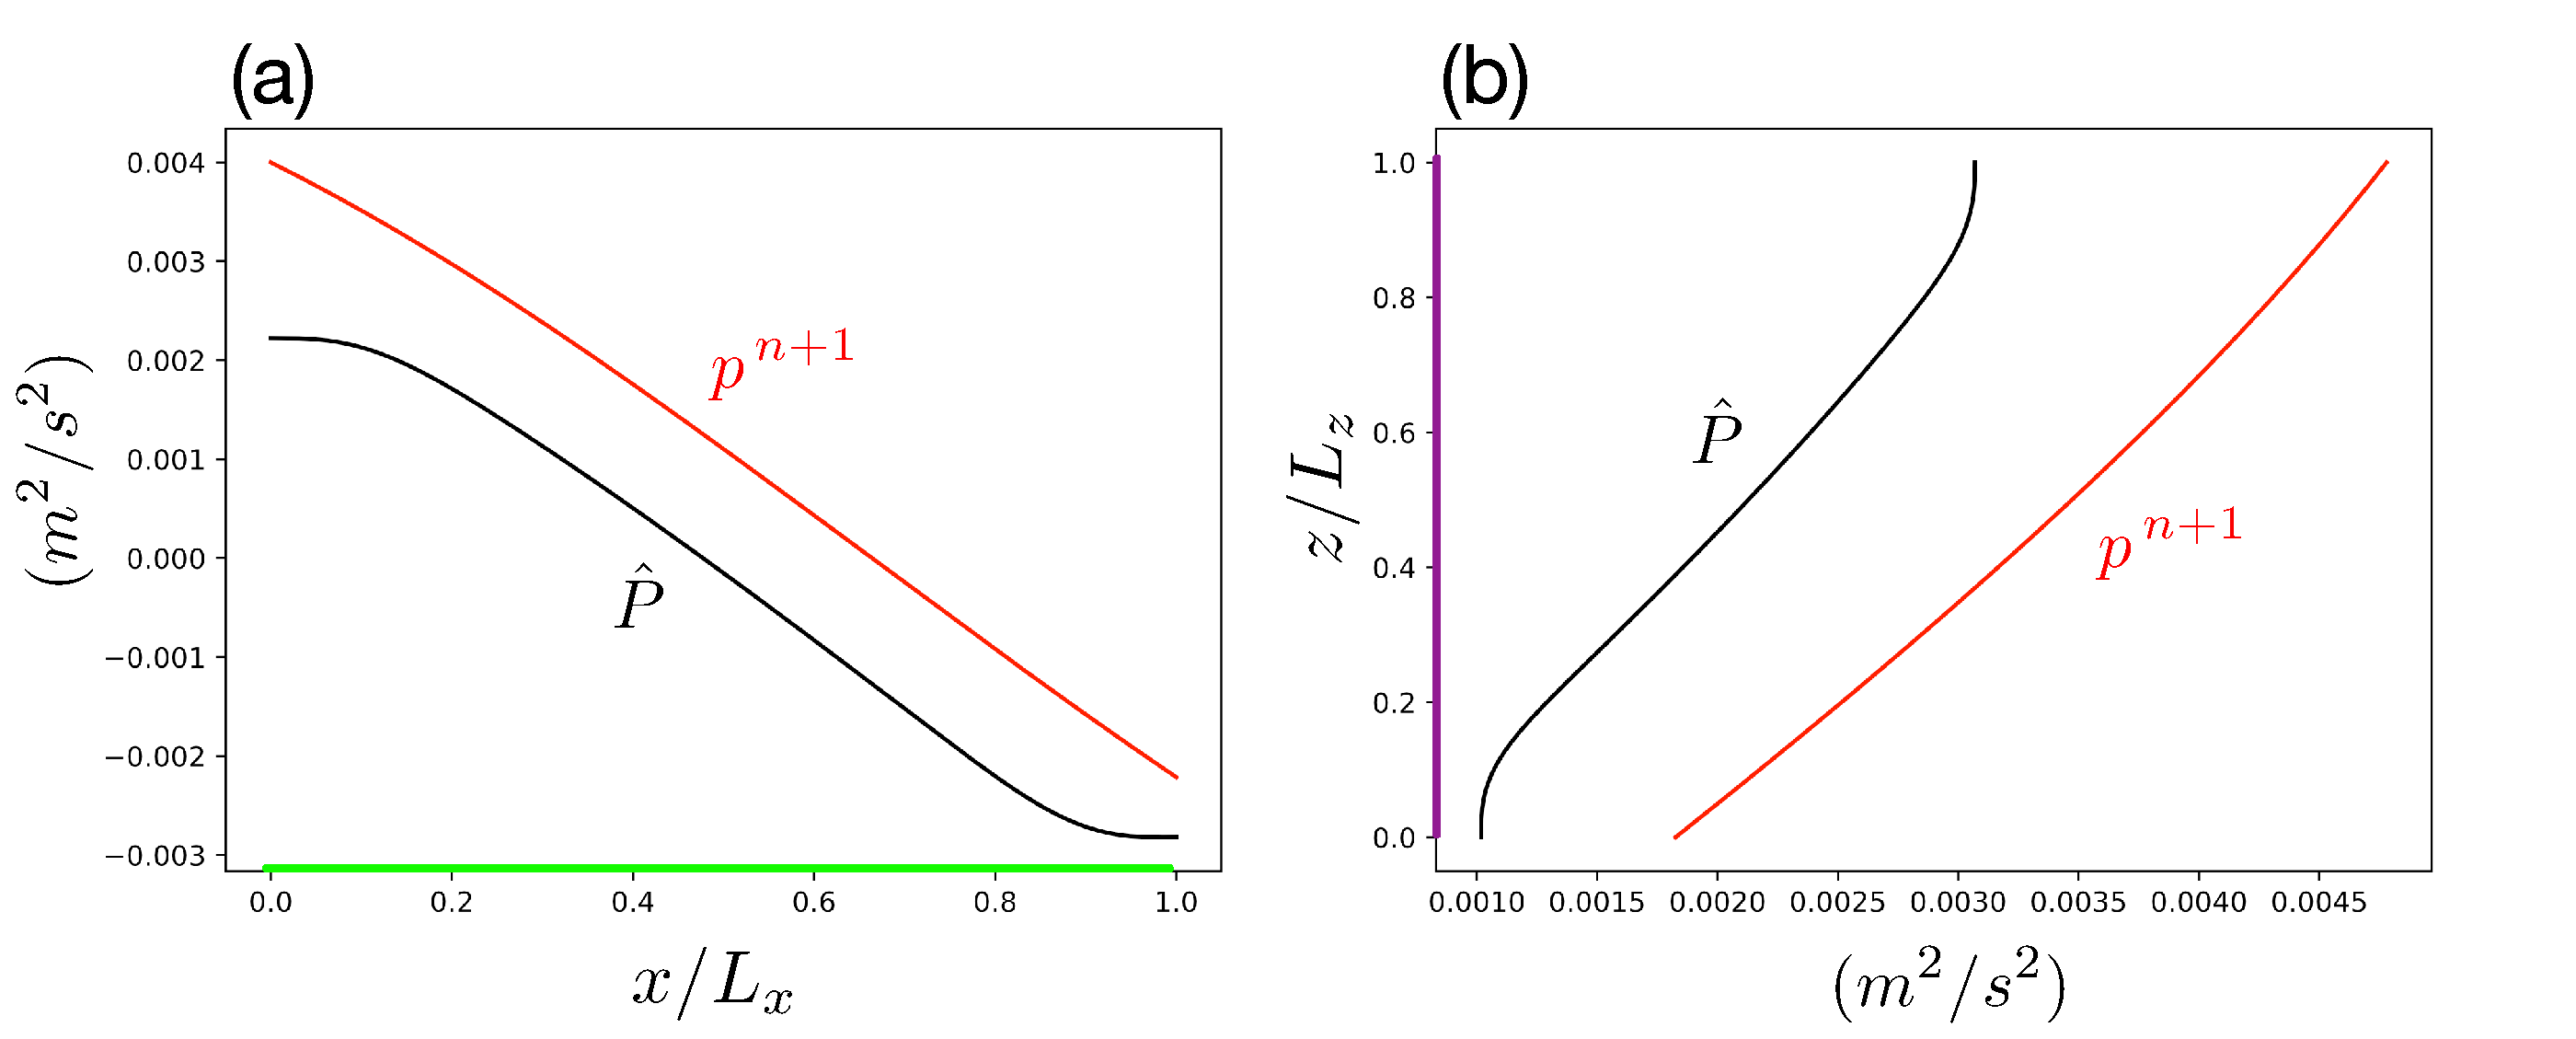
\includegraphics[width=1.0\textwidth]{FIGS/phat_p.eps}}
  \caption{The solution ${\hat P}$ to the Poisson Eq. (\ref{eq:poisson2}) with boundary conditions (\ref{eq:poissonbcs2}). Also shown is  the true pressure variable $p$ evaluated at $t^{\,n+1}$.
  }
  \label{fig:phat_p}
\end{figure}

The inclusion of $\vec \psi$, constructed using the boundary information at $t^{\,n+1}$, was designed to yield  a projection variable ${\hat P}$ with normal derivatives that vanish at the boundaries.
Figure \ref{fig:grad_P_hat} shows the computed gradient of ${\hat P}$ along the same slices shown in the previous figures. The normal gradients vanish at the boundaries but the tangential derivatives
do not.
 \begin{figure}
  \centerline{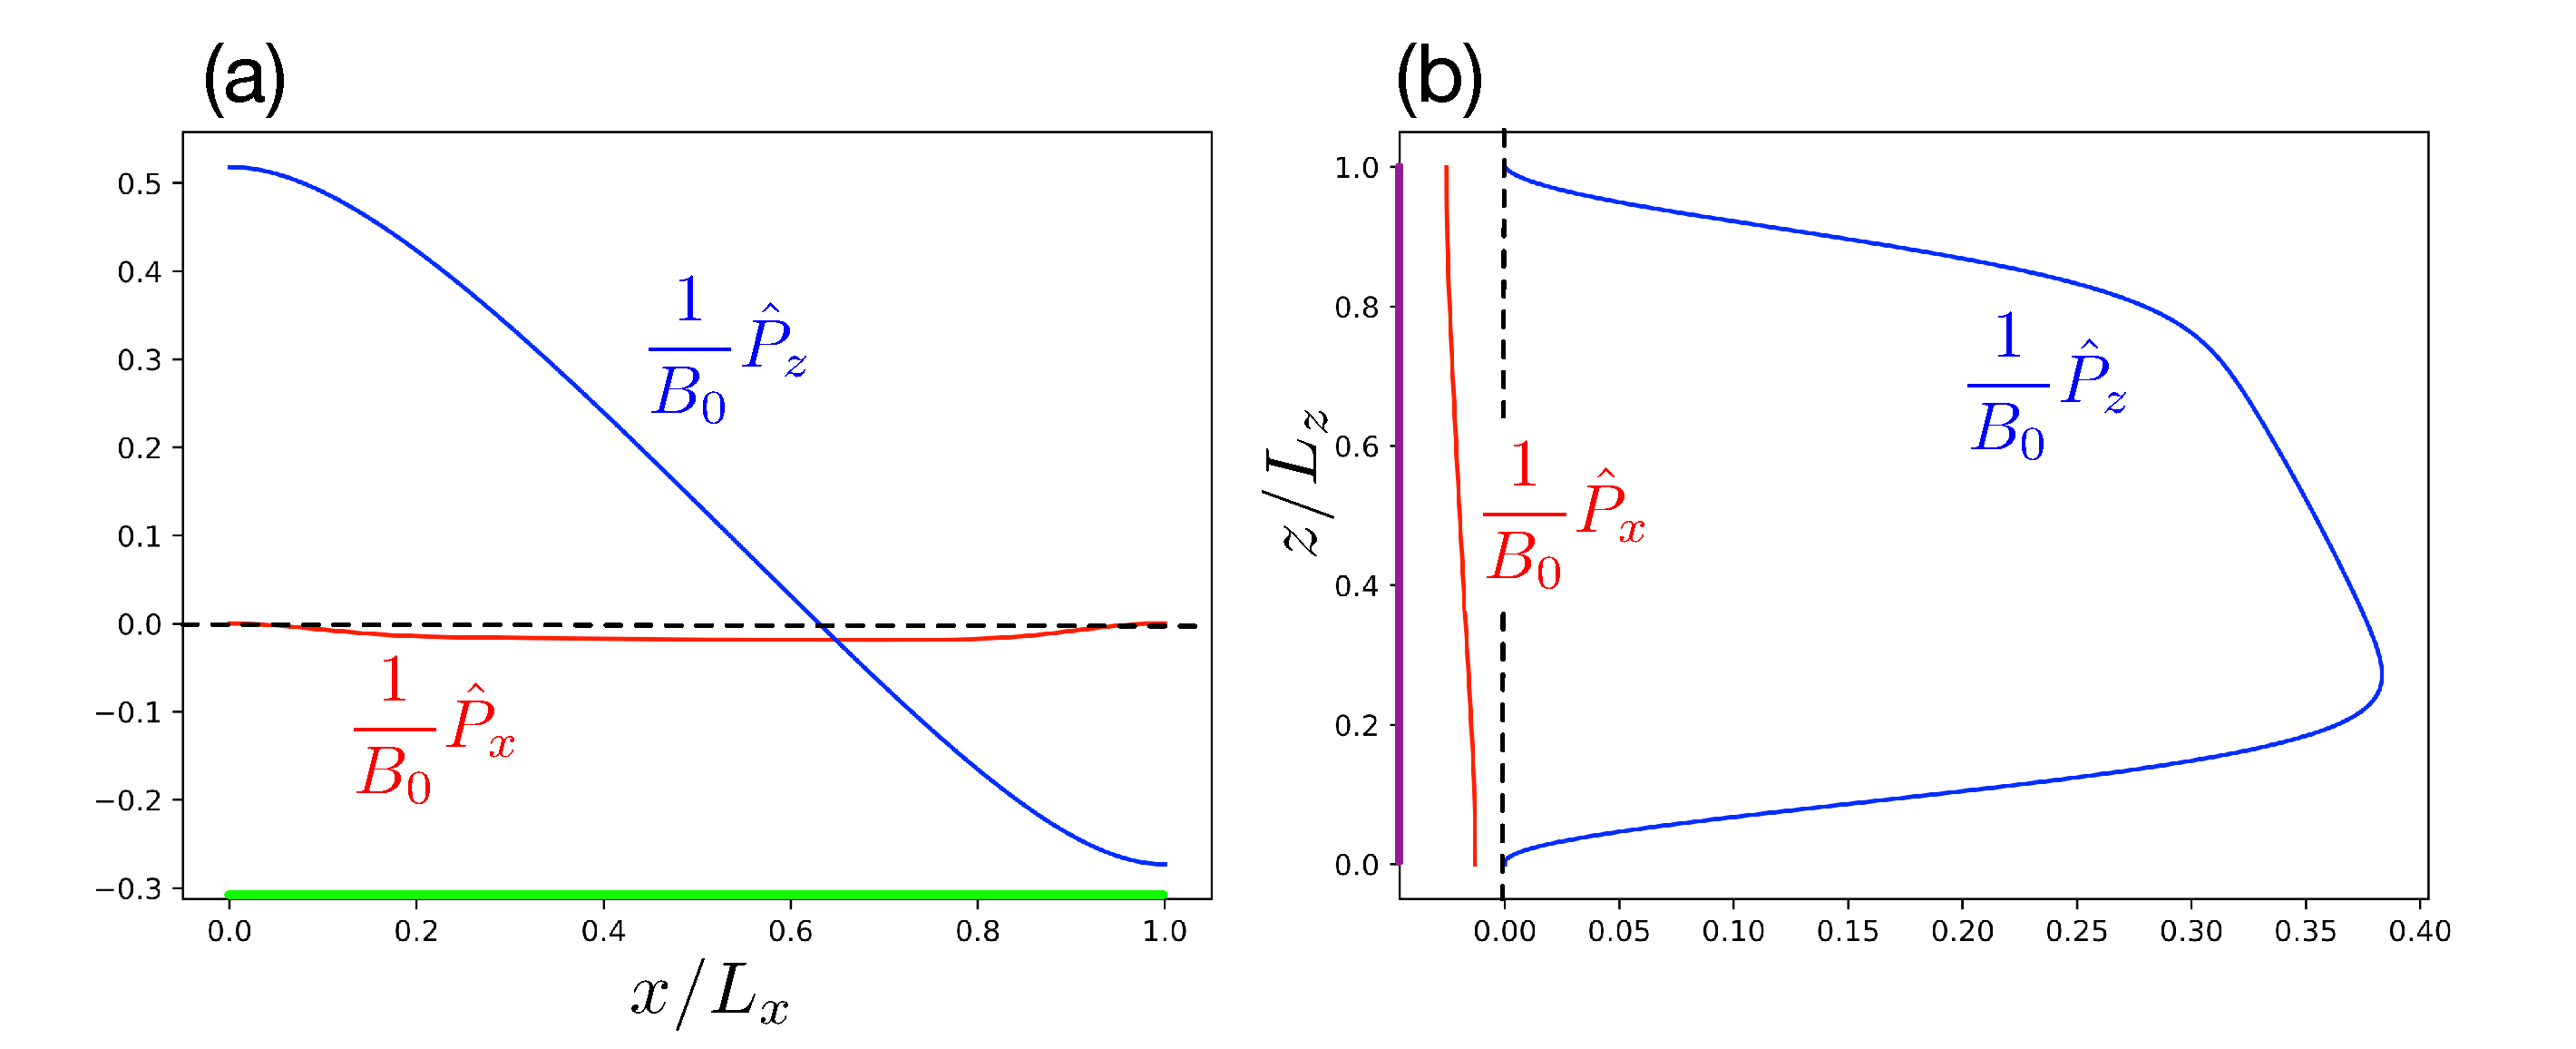
\includegraphics[width=1.0\textwidth]{FIGS/grad_P_hat.eps}}
  \caption{The gradient of the pressure variable ${\hat P}$ scaled by the maximum buoyancy perturbation $B_0 = A(k/m)(N^2/\omega)$.  Shown as (a) a function of $x$ at $z=L_z/4$ and (b) a function of $z$ at $x=L_x/4$ .
  }
  \label{fig:grad_P_hat}
\end{figure}


Finally, the computed gradient of ${\hat P}$ is used to project the intermediate variables, smoothly augmented with boundary information at $t^{\,n+1}$, onto their divergence-free subspace yielding the solutions
$u^{\,n+1}$ and $w^{\,n+1}$ via Eqs. (\ref{eq:umom6}) and (\ref{eq:wmom6}). Figure \ref{fig:exact_solns} shows the result of this projection along with the exact solutions (black dots, subsampled for clarity).
In this example, $t^n=0$ and so the discrete time stepping scheme was a single first order Euler step. Independent of the spatial treatment, this is the least accurate time step in a multi-step scheme, with an error of O($\Delta t$).
Once the integration gets underway, we use AB4 and the errors in temporal integration are O($\Delta t^4$).
 \begin{figure}
  \centerline{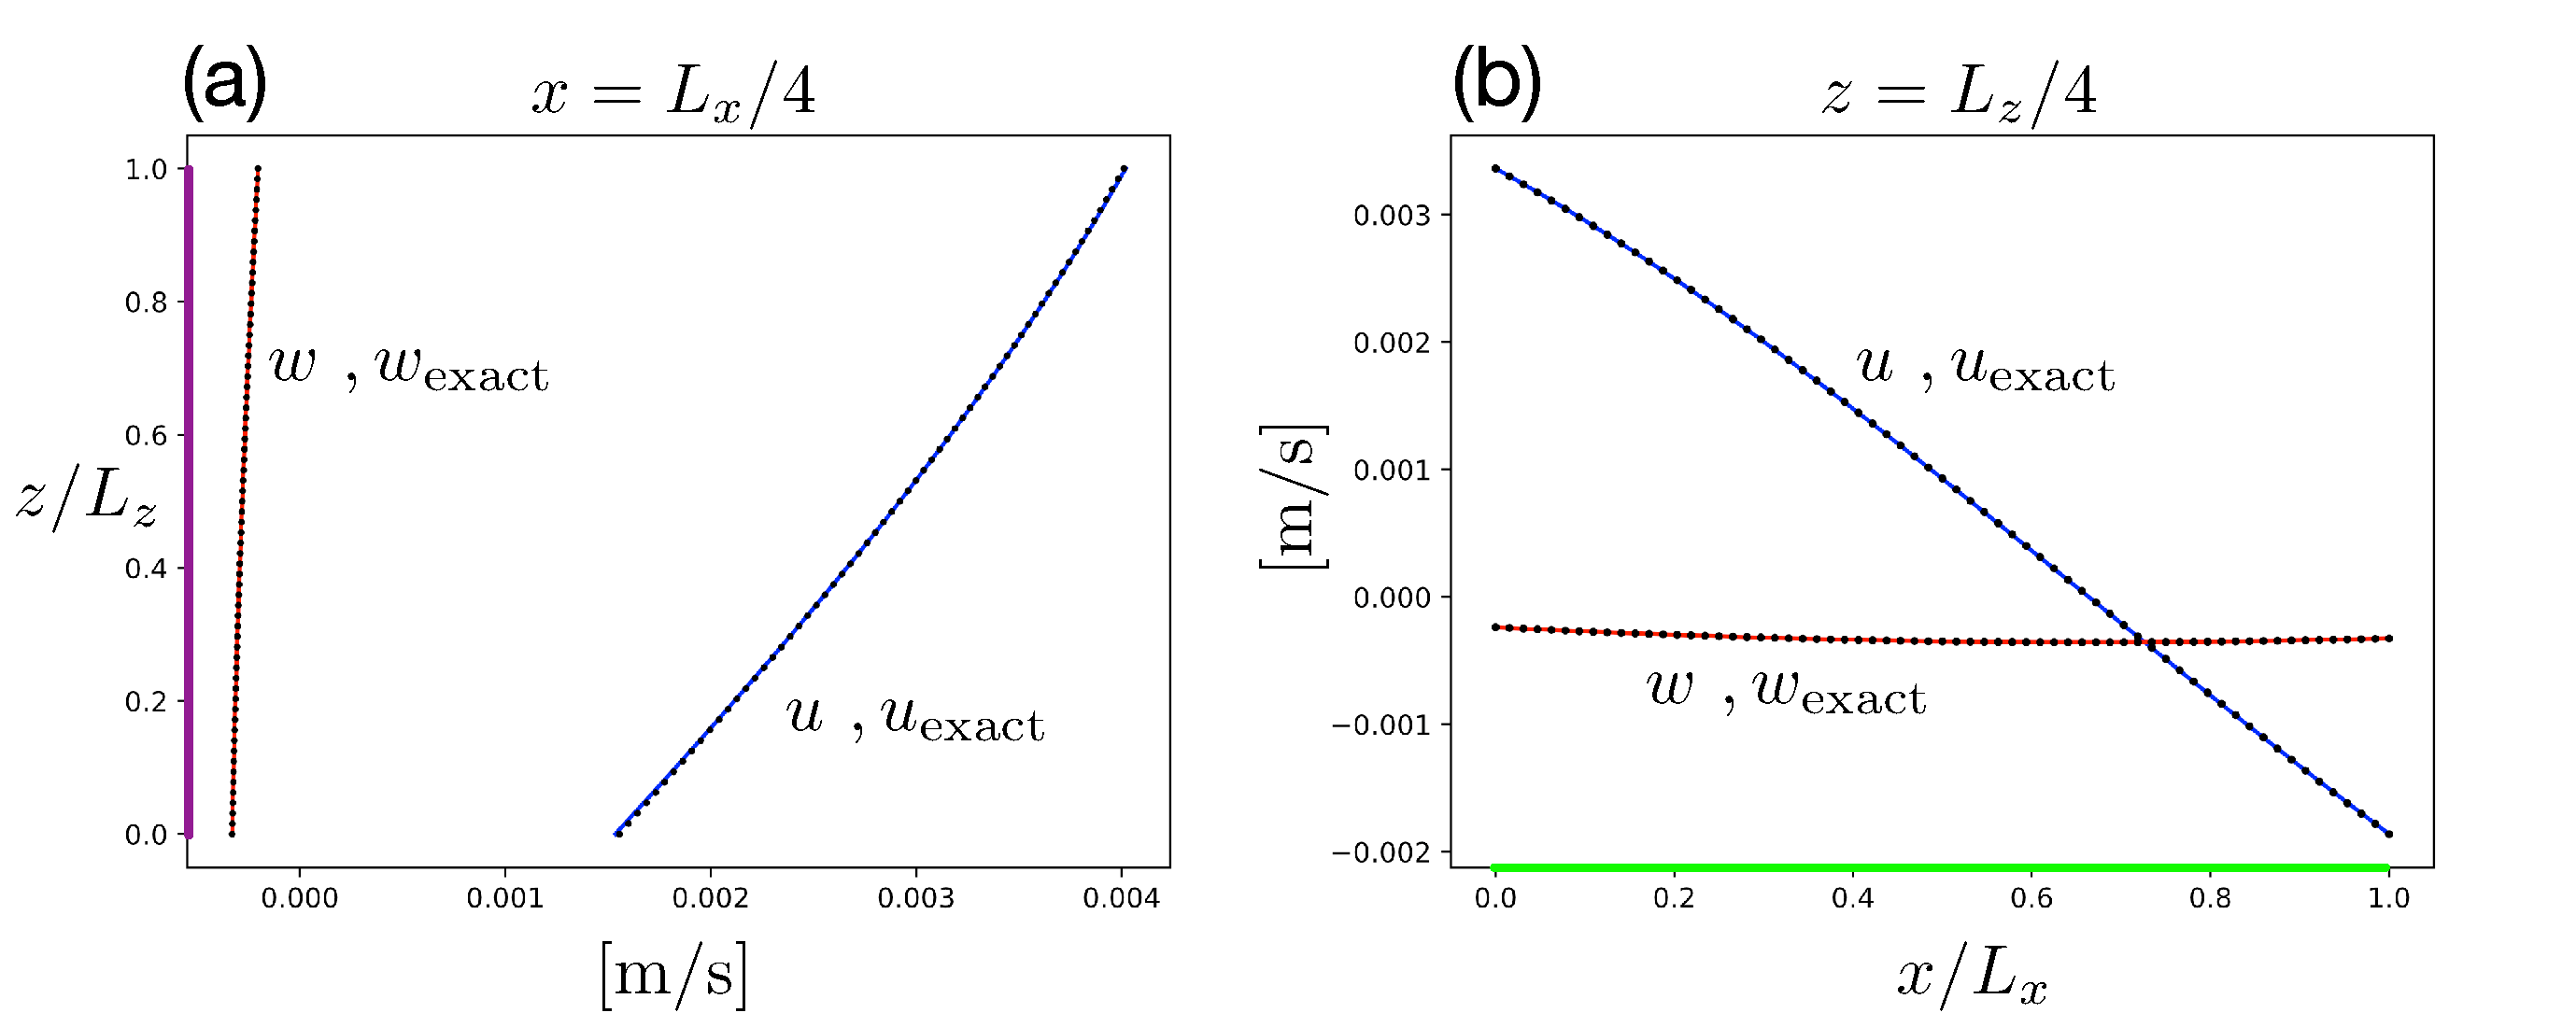
\includegraphics[width=1.0\textwidth]{FIGS/exact_solns.eps}}
  \caption{Left: Computed (black dots) and exact solutions (red)  $u^{n+1}(z)$ and $w^{n+1}(z)$ at $x=L_x/4$. Right: Computed and exact solutions  $u^{n+1}(x)$ and $w^{n+1}(x)$ at $z=L_z/4$. For the computed
  solutions, only every fourth grid point is shown.} 
  \label{fig:exact_solns}
\end{figure}

\section{Recovery of the pressure $P$}
In general, when solving for incompressible flow, the pressure itself is never required, only its gradients. Here, by construction, we never explicitly require the pressure gradients but rather
the gradients of ${\hat P}$. The gradients of $P$ (the average pressure over the time step) can, however, be recovered explicitly if desired. From Eq. (\ref{eq:umom5}) and Eq. (\ref{eq:umom6})
we see that
\begin{equation}
\nabla P = \nabla {\hat P} - \nabla \Psi
\end{equation}
where
\begin{equation}
\Delta t \, \nabla \Psi = [ \psi_u,\psi_w].
\end{equation}
The gradient of ${\hat P}$ is explicitly computed as are the boundary-matched functions $\psi_u$ and $\psi_w$. Note however, that these are never explicitly combined to form the Recovering $P$ itself, however, requires solution of a Poisson equation with inhomogeneous Neumann
conditions, precisely the problem we avoided in adopting this approach.



\section{Comments}
\begin{itemize}
\setlength\itemsep{1em}
\item Most of the work of the pressure projection seems to be focussed on recovering from the large differences between $w_*$ and $w^{\,n+1}$ induced by the buoyancy forces. I find this interesting.
\item I have not yet run multiple time steps with everything working cleanly like this!!!!!
\item ${\hat P}_x$ seems to be slightly non-zero at $x=0$ and $x=L$ despite this being formally true in the cosine transform solution procedure. In the example, the gradient of ${\hat P}$ was computed
using the Bernoulli-cosine series but perhaps it should really be done using a strictly cosine approach. I could probably add a simple switch to the routines to trigger this as desired.
\item I think this is a quite difficult test step for the algorithm. The discontinuities in derivatives over the even-extended child domain are distinct for all variables.
\item It's interesting that to formulate the problem formally, it's the tangential derivatives of the tangential velocities that are needed, not the boundary values themselves.
\item While $P$ itself is never needed in the solution algorithm, and the physically relevant vector $\nabla P$ can be easily reconstructed, it is useful to have $P$ available for calculating
the wave fluxes (pressure work) across surfaces of interest. I don't see how that can be done for problems lacking symmetry constraints without being able to solve fully inhomogeneous elliptic problems.
\item When the boundary influence functions are increasingly localized to the boundaries by taking $\gamma_x \to O(\Delta x)$ and $\gamma_z \to O(\Delta z)$, the variable ${\hat P}$ differs from $P$
only in thin boundary layers. This problem however gives rise to numerical accuracy problems and I'm finding much better solutions for $u^{\,n+1}$ and $w^{\,n+1}$ by taking $\gamma_x$ and $\gamma_z$
substantially larger.
\item This note does not address issues related to boundary conditions for outgoing signals in nested simulations.
\end{itemize}



\bibliographystyle{jfm}
% Note the spaces between the initials
\bibliography{ttbl.bib}

\end{document}
